% Figure 2 vector source (standalone; compile with -jobname=fig2_floors).
% Three escape routes (all online-LLM procedures) leave an error floor; zero-call
% compilation removes it. All in-figure text >= 9pt Helvetica; axis/tick/bar lines 0.5pt.
% Series colors: blue=Iowa&CG(ours), violet=GovTwin, teal=MultiGov, dark-red=ICT;
% red hatch = error/floor motif shared with Figure 1's contract-gap band.
\documentclass[10pt]{standalone}
\usepackage{helvet}
\usepackage{tikz}
\usepackage{pgfplots}
\pgfplotsset{compat=1.17, every axis/.append style={axis line style={line width=0.5pt}},
  every tick/.append style={line width=0.5pt, black},
  every mark/.append style={line width=0.5pt},
  error bars/error bar style={line width=0.5pt}}
\usetikzlibrary{patterns,arrows.meta}
\begin{document}
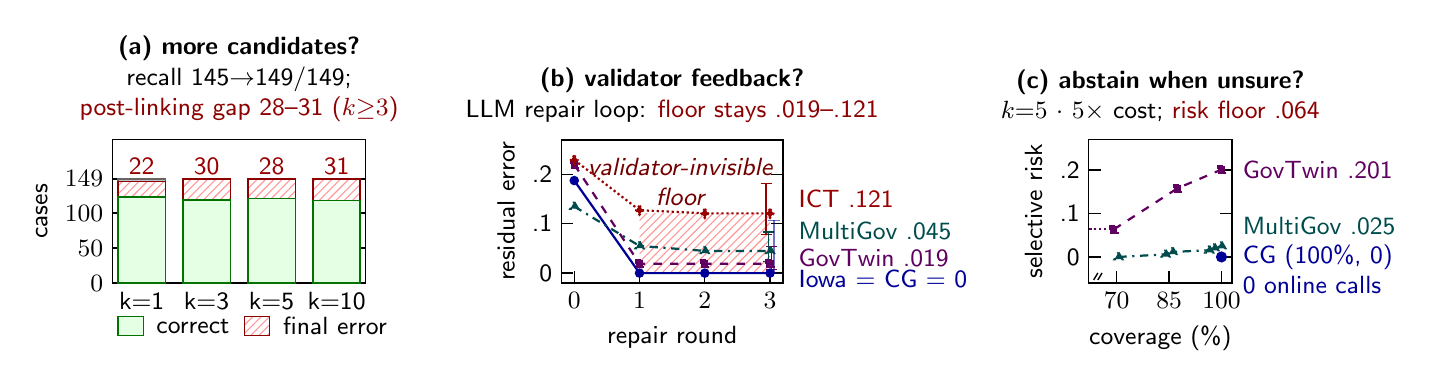
\begin{tikzpicture}
\small\sffamily
%%%%%%%%%%%%%%%% (a) candidate budget %%%%%%%%%%%%%%%%
\begin{axis}[
  at={(0mm,0mm)}, anchor=south west,
  width=48mm, height=34mm,
  title={\textbf{(a) more candidates?}\\recall 145$\to$149/149;\\{\color{red!55!black}post-linking gap 28--31 ($k{\ge}3$)}},
  title style={font=\small\sffamily, align=center, yshift=-1mm},
  ybar stacked, bar width=6mm, xtick pos=bottom,
  symbolic x coords={k=1,k=3,k=5,k=10}, xtick=data,
  ymin=0, ymax=205, ytick={0,50,100,149},
  ylabel={cases}, ylabel near ticks,
  label style={font=\small\sffamily}, tick label style={font=\small\sffamily},
  enlarge x limits=0.15,
  clip=false,
]
\addplot[fill=green!10, draw=green!45!black, line width=0.5pt] coordinates {(k=1,123) (k=3,119) (k=5,121) (k=10,118)};
\addplot[pattern=north east lines, pattern color=red!40, draw=red!55!black, line width=0.5pt] coordinates {(k=1,22) (k=3,30) (k=5,28) (k=10,31)};
\addplot[fill=black!25, draw=black!60, line width=0.5pt] coordinates {(k=1,4) (k=3,0) (k=5,0) (k=10,0)};
% per-bar final-error counts
\node[font=\small\sffamily, text=red!60!black, anchor=south, inner sep=1pt] at (axis cs:k=1,150) {22};
\node[font=\small\sffamily, text=red!60!black, anchor=south, inner sep=1pt] at (axis cs:k=3,150) {30};
\node[font=\small\sffamily, text=red!60!black, anchor=south, inner sep=1pt] at (axis cs:k=5,150) {28};
\node[font=\small\sffamily, text=red!60!black, anchor=south, inner sep=1pt] at (axis cs:k=10,150) {31};
% inline legend under the x axis
\node[fill=green!10, draw=green!45!black, minimum width=3.2mm, minimum height=2.4mm, inner sep=0pt, anchor=west] at (rel axis cs:0.02,-0.30) {};
\node[font=\small\sffamily, anchor=west, xshift=3.8mm] at (rel axis cs:0.02,-0.30) {correct};
\node[pattern=north east lines, pattern color=red!40, draw=red!55!black, minimum width=3.2mm, minimum height=2.4mm, inner sep=0pt, anchor=west] at (rel axis cs:0.52,-0.30) {};
\node[font=\small\sffamily, anchor=west, xshift=3.8mm] at (rel axis cs:0.52,-0.30) {final error};
\end{axis}
%%%%%%%%%%%%%%%% (b) validator feedback %%%%%%%%%%%%%%%%
\begin{axis}[
  at={(57mm,0mm)}, anchor=south west,
  width=44mm, height=34mm,
  title={\textbf{(b) validator feedback?}\\LLM repair loop: {\color{red!55!black}floor stays .019--.121}},
  title style={font=\small\sffamily, align=center, yshift=-1mm},
  xmin=-0.2, xmax=3.2, xtick={0,1,2,3}, xtick pos=bottom,
  ymin=-0.02, ymax=0.27, ytick={0,.1,.2}, yticklabels={0,.1,.2},
  xlabel={repair round}, ylabel={residual error},
  xlabel near ticks, ylabel near ticks,
  label style={font=\small\sffamily}, tick label style={font=\small\sffamily},
  clip=false,
]
\fill[pattern=north east lines, pattern color=red!40] (axis cs:1,0) rectangle (axis cs:3,0.121);
\addplot[blue!60!black, thick, mark=*, mark size=1.3pt] coordinates {(0,0.1875)(1,0)(2,0)(3,0)};
\addplot[violet!75!black, thick, dashed, mark=square*, mark size=1.3pt] coordinates {(0,0.2201)(1,0.0189)(2,0.0189)(3,0.0189)};
\addplot[teal!60!black, thick, dashdotted, mark=triangle*, mark size=1.6pt] coordinates {(0,0.1350)(1,0.0550)(2,0.0450)(3,0.0450)};
\addplot[red!60!black, thick, densely dotted, mark=diamond*, mark size=1.6pt] coordinates {(0,0.2293)(1,0.1274)(2,0.1210)(3,0.1210)};
\addplot[red!60!black, error bars/.cd, y dir=both, y explicit] coordinates {(2.94,0.1210) += (0,0.0603) -= (0,0.0422)};
\addplot[teal!60!black, error bars/.cd, y dir=both, y explicit] coordinates {(2.98,0.0450) += (0,0.0383) -= (0,0.0211)};
\addplot[blue!60!black, opacity=0.55, error bars/.cd, y dir=both, y explicit] coordinates {(3.06,0) += (0,0.1072) -= (0,0)};
\addplot[violet!75!black, error bars/.cd, y dir=both, y explicit] coordinates {(3.02,0.0189) += (0,0.0351) -= (0,0.0124)};
% end labels near true endpoint heights
\node[font=\small\sffamily, anchor=west, text=red!60!black] at (axis cs:3.30,0.150) {ICT .121};
\node[font=\small\sffamily, anchor=west, text=teal!60!black] at (axis cs:3.30,0.085) {MultiGov .045};
\node[font=\small\sffamily, anchor=west, text=violet!75!black] at (axis cs:3.30,0.030) {GovTwin .019};
\node[font=\small\sffamily, anchor=west, text=blue!60!black] at (axis cs:3.30,-0.012) {Iowa = CG = 0};
\node[font=\small\sffamily\itshape, align=center, text=red!45!black] at (axis cs:1.62,0.185) {validator-invisible\\floor};
\end{axis}
%%%%%%%%%%%%%%%% (c) abstention %%%%%%%%%%%%%%%%
\begin{axis}[
  at={(124mm,0mm)}, anchor=south west,
  width=34mm, height=34mm,
  title={\textbf{(c) abstain when unsure?}\\$k{=}5$ $\cdot$ $5\times$ cost; {\color{red!55!black}risk floor .064}},
  title style={font=\small\sffamily, align=center, yshift=-1mm},
  xmin=62, xmax=103, xtick={70,85,100}, xtick pos=bottom,
  ymin=-0.06, ymax=0.27, ytick={0,.1,.2}, yticklabels={0,.1,.2},
  xlabel={coverage (\%)}, ylabel={selective risk},
  xlabel near ticks, ylabel near ticks,
  label style={font=\small\sffamily}, tick label style={font=\small\sffamily},
  clip=false,
]
\addplot[violet!75!black, thick, densely dotted, domain=62:69.18] {0.0636};
\addplot[violet!75!black, thick, dashed, mark=square*, mark size=1.3pt] coordinates {(69.18,0.0636)(87.42,0.1583)(100,0.2013)};
\addplot[teal!60!black, thick, dashdotted, mark=triangle*, mark size=1.6pt] coordinates {(70.5,0)(84,0.006)(86,0.0116)(96.5,0.0155)(98,0.0204)(100,0.025)};
\addplot[only marks, mark=*, mark size=1.8pt, blue!60!black] coordinates {(100,0)};
% inline labels
\node[font=\small\sffamily, anchor=west, text=violet!75!black] at (axis cs:103.5,0.201) {GovTwin .201};
\node[font=\small\sffamily, anchor=west, text=teal!60!black] at (axis cs:103.5,0.072) {MultiGov .025};
\node[font=\small\sffamily, anchor=west, align=left, text=blue!60!black] at (axis cs:103.5,-0.028) {CG (100\%, 0)\\0 online calls};
\draw[line width=0.5pt] (axis cs:63.4,-0.053) -- (axis cs:64.6,-0.037);
\draw[line width=0.5pt] (axis cs:64.6,-0.053) -- (axis cs:65.8,-0.037);
\end{axis}
\end{tikzpicture}
\end{document}
